\documentclass[11pt,a4paper]{article}
\usepackage[utf8]{inputenc}
\usepackage[spanish]{babel}
\usepackage{amsmath}
\usepackage{amsfonts}
\usepackage{amssymb}
\usepackage{graphicx}
\usepackage{enumitem}
\usepackage{geometry}
\usepackage{float} % Paquete crítico para forzar la posición [H]

\geometry{left=2.5cm,right=2.5cm,top=2.5cm,bottom=2.5cm}

\begin{document}

% --- ENCABEZADO ---
\begin{center}
    \textbf{UNIVERSIDAD TECNOLÓGICA NACIONAL \\ FACULTAD REGIONAL LA PLATA} \\
    \vspace{0.2cm}
    \textbf{INGENIERÍA MECÁNICA - Curso 2026} \\
    \vspace{0.2cm}
    \textit{Asignatura: ESTABILIDAD 1}
\end{center}

\vspace{0.3cm}

\begin{flushleft}
    \textbf{Prof. Titular:} Ing. Augusto VAELLO \\
    \textbf{JTP:} Ing. Jorge RONCONI \\
\end{flushleft}

\noindent\rule{\linewidth}{0.4pt}

\begin{center}
    \vspace{0.4cm}
    \Large \textbf{Trabajo Práctico Nº 1: FUERZAS CONCURRENTES EN EL PLANO} \\
    \vspace{0.4cm}
\end{center}

% --- EJERCICIO 1 ---
\subsection*{Ejercicio Nº1: Resolución por Proyecciones}
Dado el sistema de fuerzas concurrentes representado en la Figura 1, determinar la resultante $\vec{R}$ considerando únicamente el subconjunto $\{F_1, F_2, F_3, F_4, F_5\}$.
\begin{enumerate}[label=\alph*)]
    \item \textbf{Analíticamente:} Calcular módulo, dirección y sentido de la resultante mediante ecuaciones de proyecciones sobre los ejes cartesianos $X$ e $Y$.
    \item \textbf{Gráficamente:} Verificar el resultado aplicando el método del polígono de fuerzas a una escala conveniente.
\end{enumerate}


% --- EJERCICIO 2 ---
\subsection*{Ejercicio Nº2: Resolución por Momentos}
Para el sistema de la Figura 1, hallar la resultante del subconjunto de fuerzas $\{F_2, F_3, F_4, F_5, F_6\}$.
\begin{enumerate}[label=\alph*)]
    \item \textbf{Analíticamente:} Plantear dos ecuaciones de momentos respecto a puntos que no pertenezcan a los ejes coordenados.
    \item \textbf{Gráficamente:} Verificar la dirección y ubicación de la recta de acción de la resultante.
\end{enumerate}


% --- EJERCICIO 3 ---
\subsection*{Ejercicio Nº3: Método Mixto}
Hallar la resultante del subconjunto de fuerzas $\{F_1, F_3, F_4, F_5, F_6\}$ indicado en la Figura 1.
\begin{enumerate}[label=\alph*)]
    \item \textbf{Analíticamente:} Resolver mediante el empleo de una ecuación de proyección y una de momentos.
    \item \textbf{Gráficamente:} Realizar la verificación escalar y geométrica correspondiente.
\end{enumerate}

\begin{figure}[H]
    \centering
    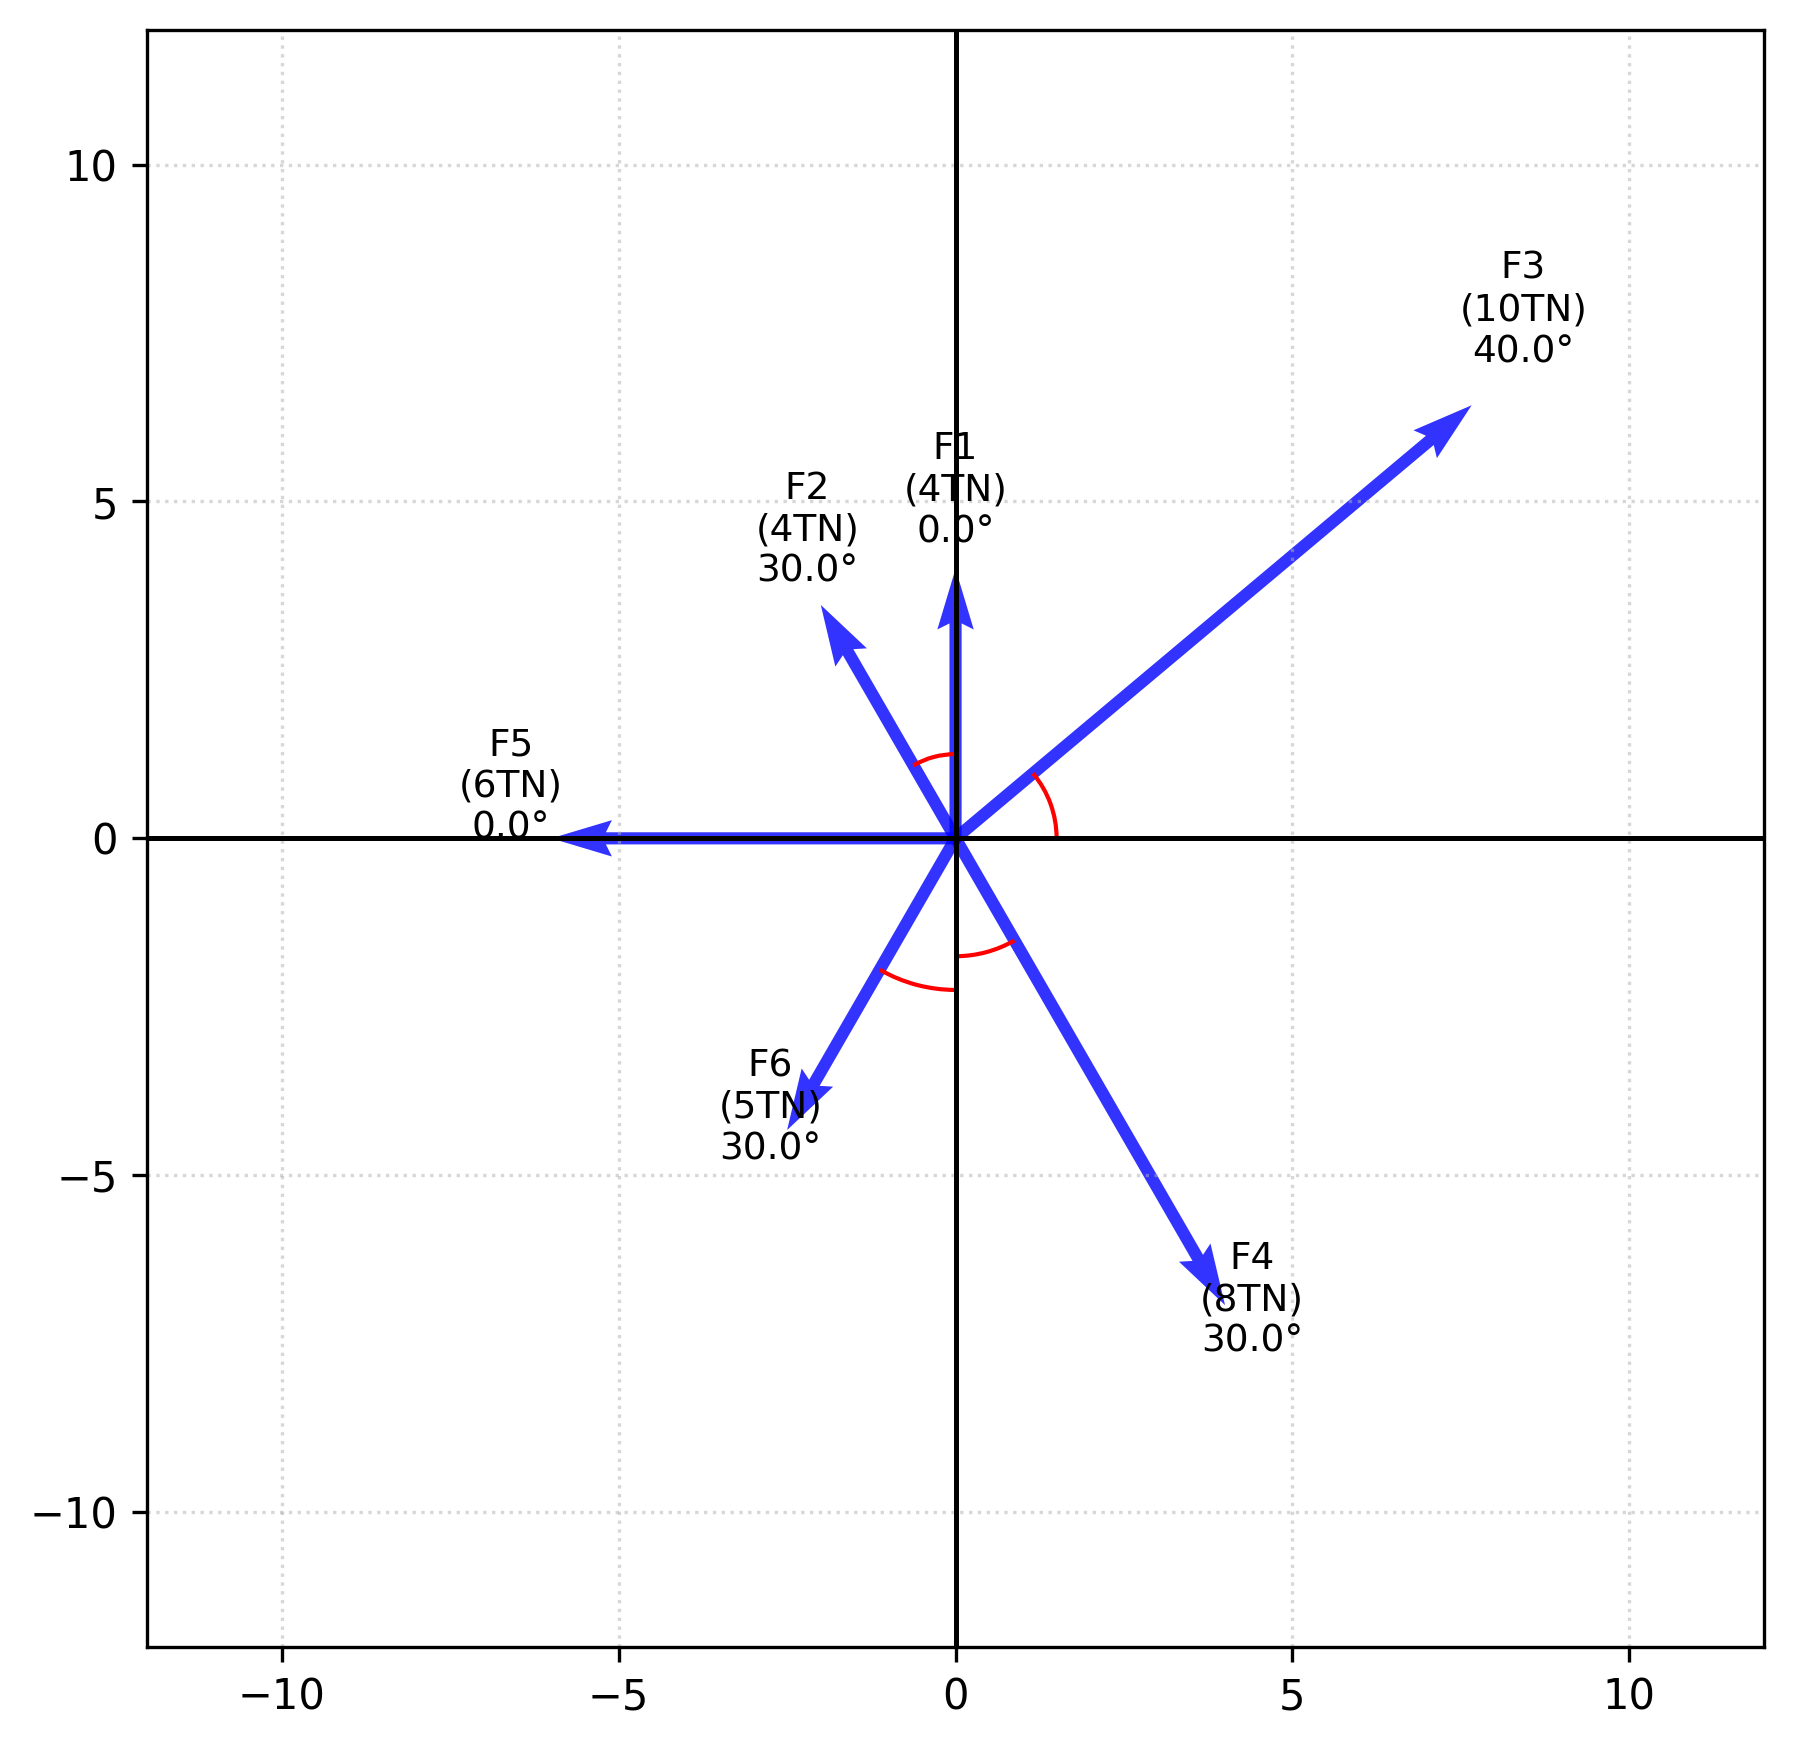
\includegraphics[width=0.7\textwidth]{img/fuerzas.png}
    \caption{Sistema de fuerzas concurrentes para los ejercicios 1, 2 y 3.}
    \label{fig:1}
\end{figure}

% --- EJERCICIO 4 ---
\subsection*{Ejercicio Nº4: Rotación del Sistema de Referencia}
Considerando la resultante obtenida en el \textbf{Ejercicio Nº1} ($\{F_1, F_2, F_3, F_4, F_5\}$):
\begin{enumerate}[label=\alph*)]
    \item \textbf{Analíticamente:} Determinar las componentes $R_{x'}$ y $R_{y'}$ referidas a una nueva terna de ejes $X' - Y'$ rotada $+45^\circ$ (sentido antihorario) respecto a la terna original. 
    \item \textbf{Verificación:} Demostrar que el módulo de la resultante $R = \sqrt{R_{x'}^2 + R_{y'}^2}$ es invariante respecto a la rotación de ejes.
\end{enumerate}


% --- EJERCICIO 5 ---
\subsection*{Ejercicio Nº5: Sistemas de Referencia No Ortogonales}
Para el sistema de fuerzas del \textbf{Ejercicio Nº2} ($\{F_2, F_3, F_4, F_5, F_6\}$):
\begin{enumerate}[label=\alph*)]
    \item \textbf{Analíticamente:} Determinar la resultante proyectando las fuerzas sobre una terna de ejes oblicuos $X'' - Y''$, donde el eje $X''$ está rotado $+40^\circ$ y el eje $Y''$ está rotado $+60^\circ$ (ambos en sentido horario respecto a la terna original). 
    \item \textbf{Discusión:} Justificar por qué las componentes ($R_{x''}, R_{y''}$) no pueden combinarse mediante el Teorema de Pitágoras para obtener el módulo.
    \item \textbf{Gráficamente:} Verificar mediante el método del paralelogramo que la suma vectorial de dichas componentes coincide con la resultante real.
\end{enumerate}

% --- EJERCICIO 6 ---
\subsection*{Ejercicio Nº6: Traslación y Par de Transporte}
Tomar la resultante hallada en el \textbf{Ejercicio Nº3} y realizar las siguientes operaciones (ver Figura 2):
\begin{enumerate}[label=\alph*)]
    \item Descomponer la resultante en las direcciones dadas: $a$ (a $30^\circ$) y $b$ (a $140^\circ$).
    \item Trasladar la resultante a los puntos $A(-4, 1)$ m y $B(2, 3)$ m, determinando en cada caso el par de transporte necesario para mantener la equivalencia del sistema.
\end{enumerate}

\begin{figure}[H]
    \centering
    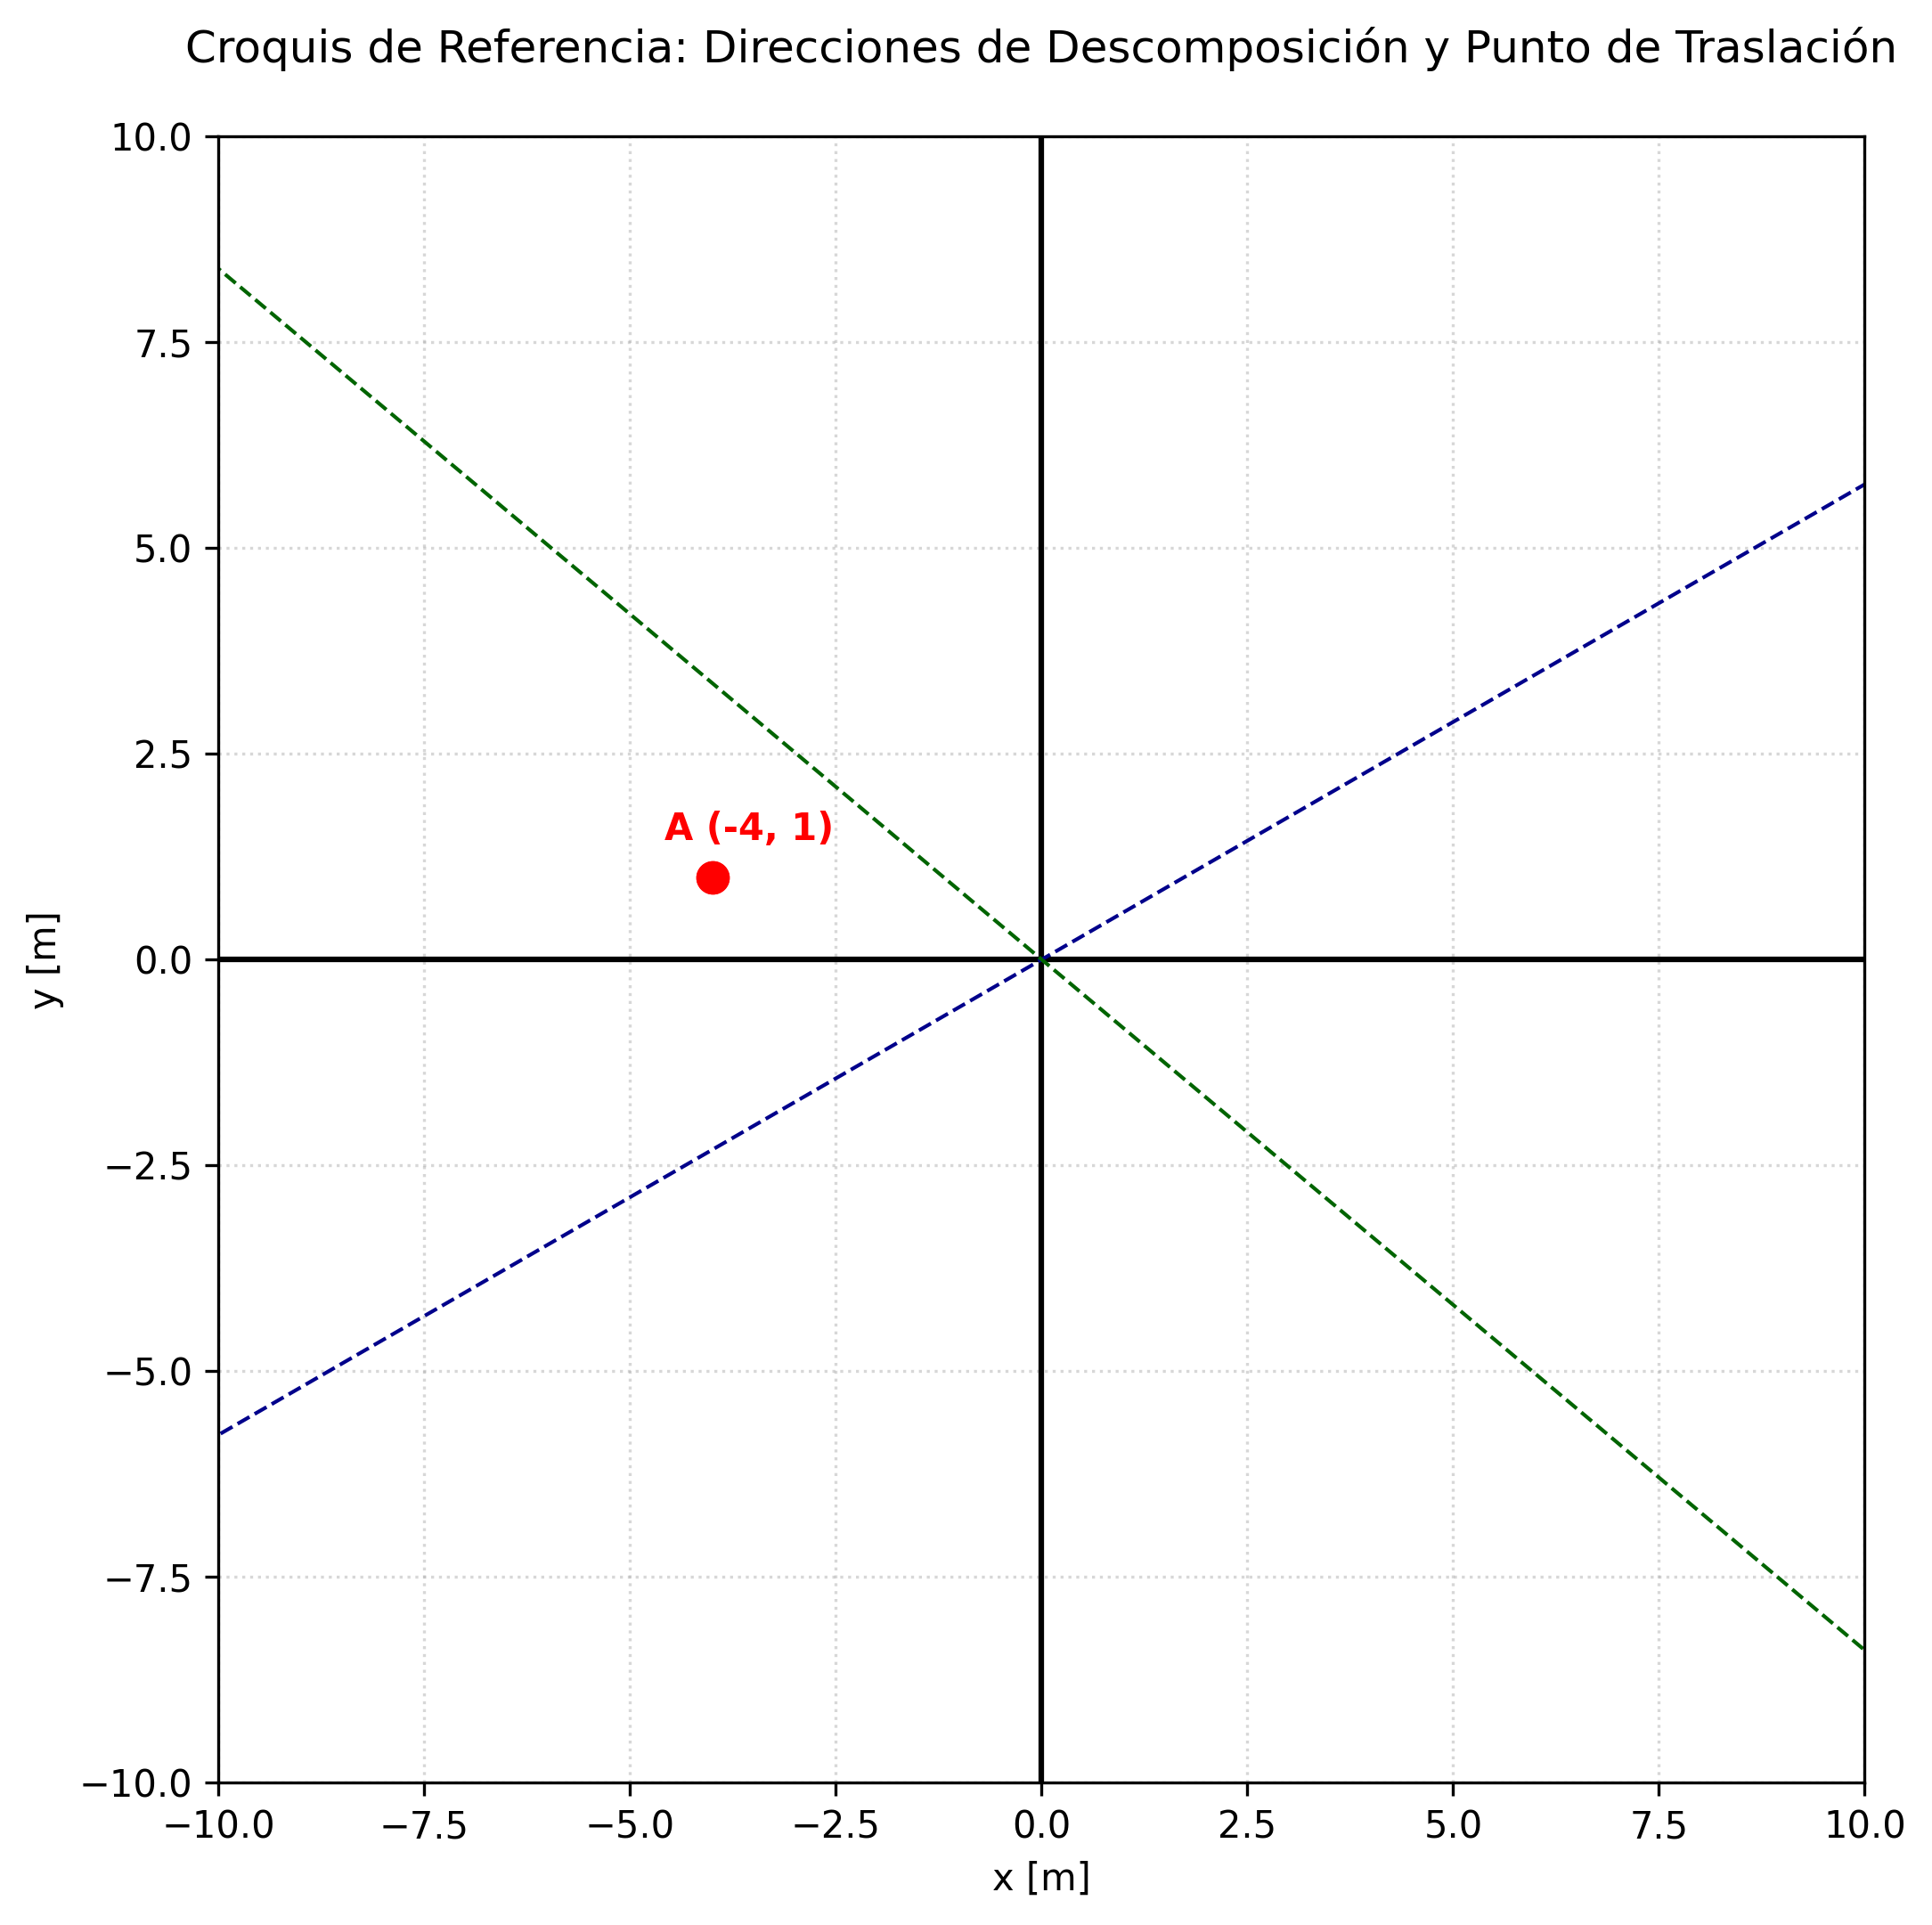
\includegraphics[width=0.7\textwidth]{img/croquis_referencia.png}
    \caption{Croquis de Referencia: Direcciones y Puntos de Traslación.}
    \label{fig:2}
\end{figure}

% --- EJERCICIO 7 ---
\subsection*{Ejercicio Nº7: Equilibrio en el Plano}
En un nudo de una estructura de soporte, se encuentra suspendido un semáforo de peso $P = 0,125 \, \text{kN}$. El dispositivo cuelga de un cable vertical unido a otros dos cables fijos a un soporte superior que forman ángulos de $37^\circ$ y $53^\circ$ con la horizontal (Figura 3).
\begin{enumerate}[label=\alph*)]
    \item \textbf{Analíticamente:} Determinar la magnitud de la tracción en los tres cables para que el sistema esté en equilibrio ($\sum \vec{F} = 0$).
    \item \textbf{Gráficamente:} Verificar el equilibrio mediante un polígono de fuerzas cerrado.
\end{enumerate}

% --- FIGURA 3 FORZADA ---
\begin{figure}[H]
    \centering
    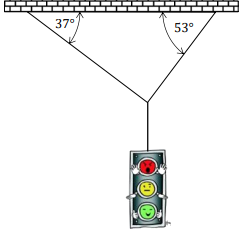
\includegraphics[width=0.6\textwidth]{img/semaforo.png}
    \caption{Esquema de semáforo en equilibrio.}
    \label{fig:3}
\end{figure}

% --- EJERCICIO 8 ---
\subsection*{Ejercicio Nº8: Determinación de la Equilibrante}
Para los sistemas definidos anteriormente, determinar el vector equilibrante $\vec{E}$:
\begin{enumerate}[label=\textbf{Sistema \arabic*:}, leftmargin=2.5cm]
    \item Hallar analíticamente la equilibrante $\vec{E}_1$ del conjunto del Ejercicio 1 y verificar gráficamente el cierre del polígono.
    \item Determinar la equilibrante $\vec{E}_2$ del conjunto del Ejercicio 2 mediante el método de momentos, verificando que $\sum M = 0$ respecto a un punto arbitrario.
    \item Calcular la equilibrante $\vec{E}_3$ del conjunto del Ejercicio 3 mediante el método mixto.
\end{enumerate}


% --- EJERCICIO 9 ---
\subsection*{Ejercicio Nº9: Variación del Momento y Teorema de Varignon}
Considerando la resultante $\vec{R}$ obtenida en el \textbf{Ejercicio Nº1}:
\begin{enumerate}[label=\alph*)]
    \item Calcular el momento de dicha resultante respecto a un punto genérico $P(0, y)$ del eje de ordenadas.
    \item Determinar la coordenada $y_P$ para la cual el momento resultante sea de $20 \, \text{kN} \cdot \text{m}$ (sentido horario).
    \item Verificar el resultado aplicando el \textit{Teorema de Varignon} con las fuerzas individuales.
\end{enumerate}

\end{document}